\documentclass[11pt]{article}
% Adapted from an original template by Hlyni Arnórssyni,
% Reykjavik University, Iceland

% ------------------------------ PAGE SETTINGS ------------------------------
\usepackage{geometry}

\geometry{
    paper=a4paper,
    top=2.5cm,
    bottom=2.5cm,
    left=2.5cm,
    right=2.4cm,
    headheight=0.75cm,
    footskip=1.5cm,
    headsep=0.75cm
}

% ------------------------------ BASIC PACKAGES ------------------------------
\usepackage{blindtext}

% Character encoding
\usepackage[T1]{fontenc}
\usepackage[utf8]{inputenc}

% Mathematics
\usepackage{amsmath, amsfonts, amsthm, amssymb}
\usepackage{braket, nicefrac}

% SI units
\usepackage{siunitx}

% Lists / columns
\usepackage{enumitem, multicol}

% ------------------------------ FIGURES ------------------------------
\usepackage{graphicx}
\usepackage{float}
\usepackage{keystroke}
\usepackage{pgfplots}
\usepgfplotslibrary{units}
\pgfplotsset{compat=1.16}

% Search these locations automatically for figures
\graphicspath{{fig/}{graphics/}{Graphics/}{./}}

% ------------------------------ TABLES ------------------------------
\usepackage{tabularx}
\usepackage{array}
\usepackage[table]{xcolor}

% ------------------------------ TYPOGRAPHY ------------------------------
\usepackage{caption}
\usepackage{titlesec}
\usepackage{microtype}
\usepackage{csquotes}

% ------------------------------ COLORS ------------------------------
\definecolor{GWBlue}{HTML}{1E4E79}

% ------------------------------ SECTION STYLING ------------------------------
\titleformat{\section}
  {\Large\bfseries\color{GWBlue}}
  {\thesection.}
  {0.40em}
  {}

\titlespacing*{\section}
  {0pt}
  {0.70em}
  {0.28em}

% ------------------------------ CAPTION STYLING ------------------------------
\captionsetup{
    font=small,
    labelfont=bf,
    textfont=it,
    labelsep=period,
    skip=4pt
}

% ------------------------------ PARAGRAPH SPACING ------------------------------
\setlength{\parindent}{0pt}
\setlength{\parskip}{0.30em}

% ------------------------------ BIBLIOGRAPHY ------------------------------
\usepackage[
    backend=biber,
    style=authoryear,
    sorting=none,
    giveninits=true,
    maxbibnames=99,
    dashed=false
]{biblatex}

\addbibresource{references.bib}

\DeclareNameAlias{sortname}{family-given}
\DeclareNameAlias{default}{family-given}
\DeclareFieldFormat[article]{title}{#1}
\DeclareFieldFormat[misc]{title}{#1}
\renewbibmacro{in:}{}

\AtEveryBibitem{%
    \clearfield{doi}%
    \clearfield{urldate}%
}

\AtBeginBibliography{\small}
\setlength{\bibitemsep}{0.35em}

% ------------------------------ HYPERLINKS ------------------------------
\usepackage{hyperref}

\hypersetup{
    colorlinks=true,
    linkcolor=GWBlue,
    citecolor=GWBlue,
    urlcolor=GWBlue
}
\usepackage{booktabs}
\setlength{\emergencystretch}{2em}
\newcommand{\srcid}[1]{\texttt{\detokenize{#1}}}
\begin{document}

% Cover page: abstract begins on page 2.
\begin{titlepage}
\centering
\vspace*{0.22\textheight}

\includegraphics[width=0.27\textwidth]{gwu_logo.pdf}\par\vspace{6pt}
{\LARGE\bfseries Where Do Neural Networks Fail?\par}
{\large\bfseries Post-Training Error Geography, Novelty Detection, and Guided Retraining with Neural Network Self-Organizing Maps\par}
\vspace{8pt}
{\normalsize Fyrooz Khan and Nazish Atta\par}
{\small Data Science Program, The George Washington University, Washington, DC\par}
{\small DATS 6501 Capstone, Fall 2026; supervised by Dr. Amir Jafari\par}
\vfill
\end{titlepage}

\begin{abstract}
High classification accuracy can obscure systematic errors that aggregate evaluation metrics cannot localize in a model's learned representation. We investigate Neural Network Self-Organizing Maps (NNSOM) as a post-training framework for mapping convolutional neural network (CNN) errors, detecting out-of-distribution (OOD) inputs, and selecting examples for targeted retraining. A LeNet-5 model trained on MNIST provides 84-dimensional embeddings organized by a $15\times15$ self-organizing map (SOM). We analyze map purity, best-matching-unit distances, U-Matrix structure, and spatial error concentration against null controls and conventional baselines. The original CNN achieves 99.18\% MNIST test accuracy; the SOM attains 98.19\% validation purity. On 10,500 MNIST validation and 26,032 SVHN OOD images, SOM quantization error achieves AUROC 0.9811, below maximum-softmax scoring (0.9985) and energy scoring (0.9998). In a separate five-seed retraining experiment, SOM-guided augmentation reduces mean test error on prespecified hotspot regions from 11.4\% to 7.8\%, while mean overall accuracy rises from 99.11\% to 99.21\%. Confidence-guided augmentation remains competitive and SOM-guided curriculum learning does not improve performance. Re-trained maps show reduced hotspot errors relative to standard training, without clear improvement in neuron purity. These results support the SOM as an interpretable tool for locating CNN failure regions and organizing targeted interventions on MNIST, rather than as a superior general-purpose detector or example-selection rule.
\par\smallskip\noindent\textbf{Keywords:} self-organizing maps; NNSOM; CNN error analysis; novelty detection; quantization error; error hotspots; targeted augmentation.
\end{abstract}

\section{Introduction}\label{sec:intro}
A classifier can attain high test accuracy while making recurring, structured mistakes. Aggregate measures, including accuracy and macro-F1, show how often predictions are correct but give little indication of where the errors lie in a network's learned feature space. A confusion matrix identifies which labels are confused, yet does not show whether those observations occupy compact, ambiguous or remote regions of the representation. These distinctions matter when deciding whether to inspect failure modes, flag unfamiliar inputs, or select examples for further training.

Local explanation techniques such as saliency maps, LIME, and SHAP examine the relationship between an individual input and a prediction \parencite{simonyan2014saliency,ribeiro2016lime,lundberg2017shap}. Their purpose differs from a population-level map of error geography. A self-organizing map (SOM) organizes high-dimensional observations onto an ordered low-dimensional grid \parencite{kohonen1990som}. Applied to the internal features of a fixed CNN, it can expose relationships among class regions, errors, and novel inputs without modifying the original classifier's inference rule.

We study this setting using LeNet-5 \parencite{lecun1998gradient} and the NNSOM implementation \parencite{jafari_nnsom}. The original MNIST-trained network supplies 84-dimensional \texttt{fc2} embeddings. A $15\times15$ SOM then provides 225 topologically organized prototypes. We examine whether errors concentrate in particular map cells; whether map-derived novelty scores separate MNIST validation inputs from the external SVHN set; and whether using map-identified hard training examples benefits subsequent CNN training. The questions form a connected study of \emph{diagnosis, detection and intervention}, not three separate models or phase reports.

Our contributions are fourfold. First, we give an end-to-end account of the frozen-CNN-to-NNSOM analysis workflow and its visualization and evaluation protocol. Second, we quantify error geography with a held-out hotspot-concentration analysis and compare the SOM with k-means, local-neighbor impurity and classifier confidence. Third, we compare quantization-error and U-Matrix novelty scores against established OOD baselines, including statistical uncertainty and diagnostic limitations. Fourth, we evaluate SOM-guided curriculum and targeted augmentation with matched controls and five-seed comparisons, then analyze SOMs fitted to the resulting CNN representations. Rather than arguing that the SOM dominates the numerical baselines, we examine what the spatial map makes understandable when simpler scores perform as well or better.

\section{Background and Related Work}\label{sec:related}
\textbf{CNN representations.} LeNet-5 established convolutional feature extraction and end-to-end learning as a practical approach to handwritten-character recognition \parencite{lecun1998gradient}. Its intermediate activations encode distinctions useful for classification without necessarily exposing the locations of residual errors. Here LeNet-5 is an experimental starting point, not a newly proposed classifier. Rather than changing its architecture, we examine its fixed 84-dimensional representation and subsequently assess whether selected training examples can improve the classifier. This separation lets us study representation geometry independently of the original prediction rule.

\textbf{Self-organizing maps and representation learning.} Kohonen introduced the SOM as a competitive-learning method that arranges learned prototypes on a low-dimensional neighborhood structure \parencite{kohonen1990som}. Its spatial organization makes distances and prototype neighborhoods inspectable, although preserving topology does not guarantee that classifier errors will separate cleanly. Vesanto and Alhoniemi investigated how trained SOM units can be clustered for interpretation \parencite{vesanto2000clustering}; our analysis instead overlays class composition, prediction errors and novelty assignments on the same grid. We use the NNSOM implementation and project-specific batch-training utilities \parencite{jafari_nnsom}, and distinguish the native package from the training update actually used for the saved map.

SOM-VAE incorporates a discrete topological representation into a learned latent-variable model \parencite{fortuin2019somvae}, while deep embedded SOM approaches jointly shape neural representations and map structure \parencite{forest2021desom}. Those methods make the embedding and map jointly adaptive. Our original diagnostic map is fitted \emph{after} a trained CNN and leaves its inference function unchanged. A later, separately evaluated retraining intervention changes the CNN through example selection rather than imposing a SOM loss during original classification training.

\textbf{Understanding systematic errors.} Gradient saliency highlights local sensitivity of a model output to input pixels \parencite{simonyan2014saliency}. LIME constructs a local surrogate explanation around one prediction \parencite{ribeiro2016lime}; SHAP attributes a prediction to input features under an additive explanation framework \parencite{lundberg2017shap}. These approaches explain individual decisions and are not substitutes for measuring the distribution of mistakes over a complete feature space. Domino uses cross-modal embeddings to reveal underperforming data slices \parencite{eyuboglu2022domino}, and the Spotlight identifies coherent regions of elevated model error \parencite{deon2022spotlight}. Our related objective differs in its reusable, explicitly topological coordinate system: the same BMU assignment indexes dominant labels, purity, erroneous predictions and OOD occupancy. We benchmark this representation against simpler error-prediction rules instead of assuming that visual structure yields superior discrimination.

\textbf{Novelty detection and simple baselines.} Hendrycks and Gimpel established maximum-softmax probability (MSP) as a useful reference for uncertainty and OOD ranking, while noting that high classifier confidence need not imply familiarity \parencite{hendrycks2017baseline}. Energy scoring aggregates logit information into a different scalar reference that can improve OOD separation \parencite{liu2020energy}. Mahalanobis scoring models class-conditional feature distributions \parencite{lee2018mahalanobis}, whereas deep nearest-neighbor approaches measure proximity to a training feature bank \parencite{sun2022knn}. None of these scalar scores intrinsically provides the fixed prototype-neighborhood view used here to relate failures across tasks. We additionally retain historical Isolation Forest, One-Class SVM and reconstruction-autoencoder comparisons as recorded. Their fitting budgets and preprocessing were not identical, and a later standardized-autoencoder analysis is explicitly exploratory rather than a retroactive replacement of the original benchmark.

\section{Methodology}\label{sec:methods}
\subsection{Data, baseline network and feature extraction}
MNIST contains 70,000 grayscale handwritten-digit images in ten classes. The recorded stratified split uses 49,000 training, 10,500 validation and 10,500 test images. A LeNet-5 CNN is trained with Adam; checkpoint selection uses validation accuracy \parencite{kingma2015adam}. The original reported evaluation gives 10,414 correct test classifications and 86 errors. For each input $x$, the feature extractor produces a vector $h(x)\in\mathbb{R}^{84}$ from \texttt{fc2}. Scaling parameters are fitted using training embeddings alone, and the scaled representation $z(x)$ is used for SOM training and scoring. Validation embeddings support diagnostic comparisons; final test predictions are not used to fit the original SOM.

Figure~\ref{fig:workflow} summarizes the actual workflow. The SOM identifies training regions and supplies \emph{selection information} for subsequent CNN retraining. It is not an extra preprocessing layer placed in front of the CNN for ordinary test-time classification.

\begin{figure}[htbp]
\centering
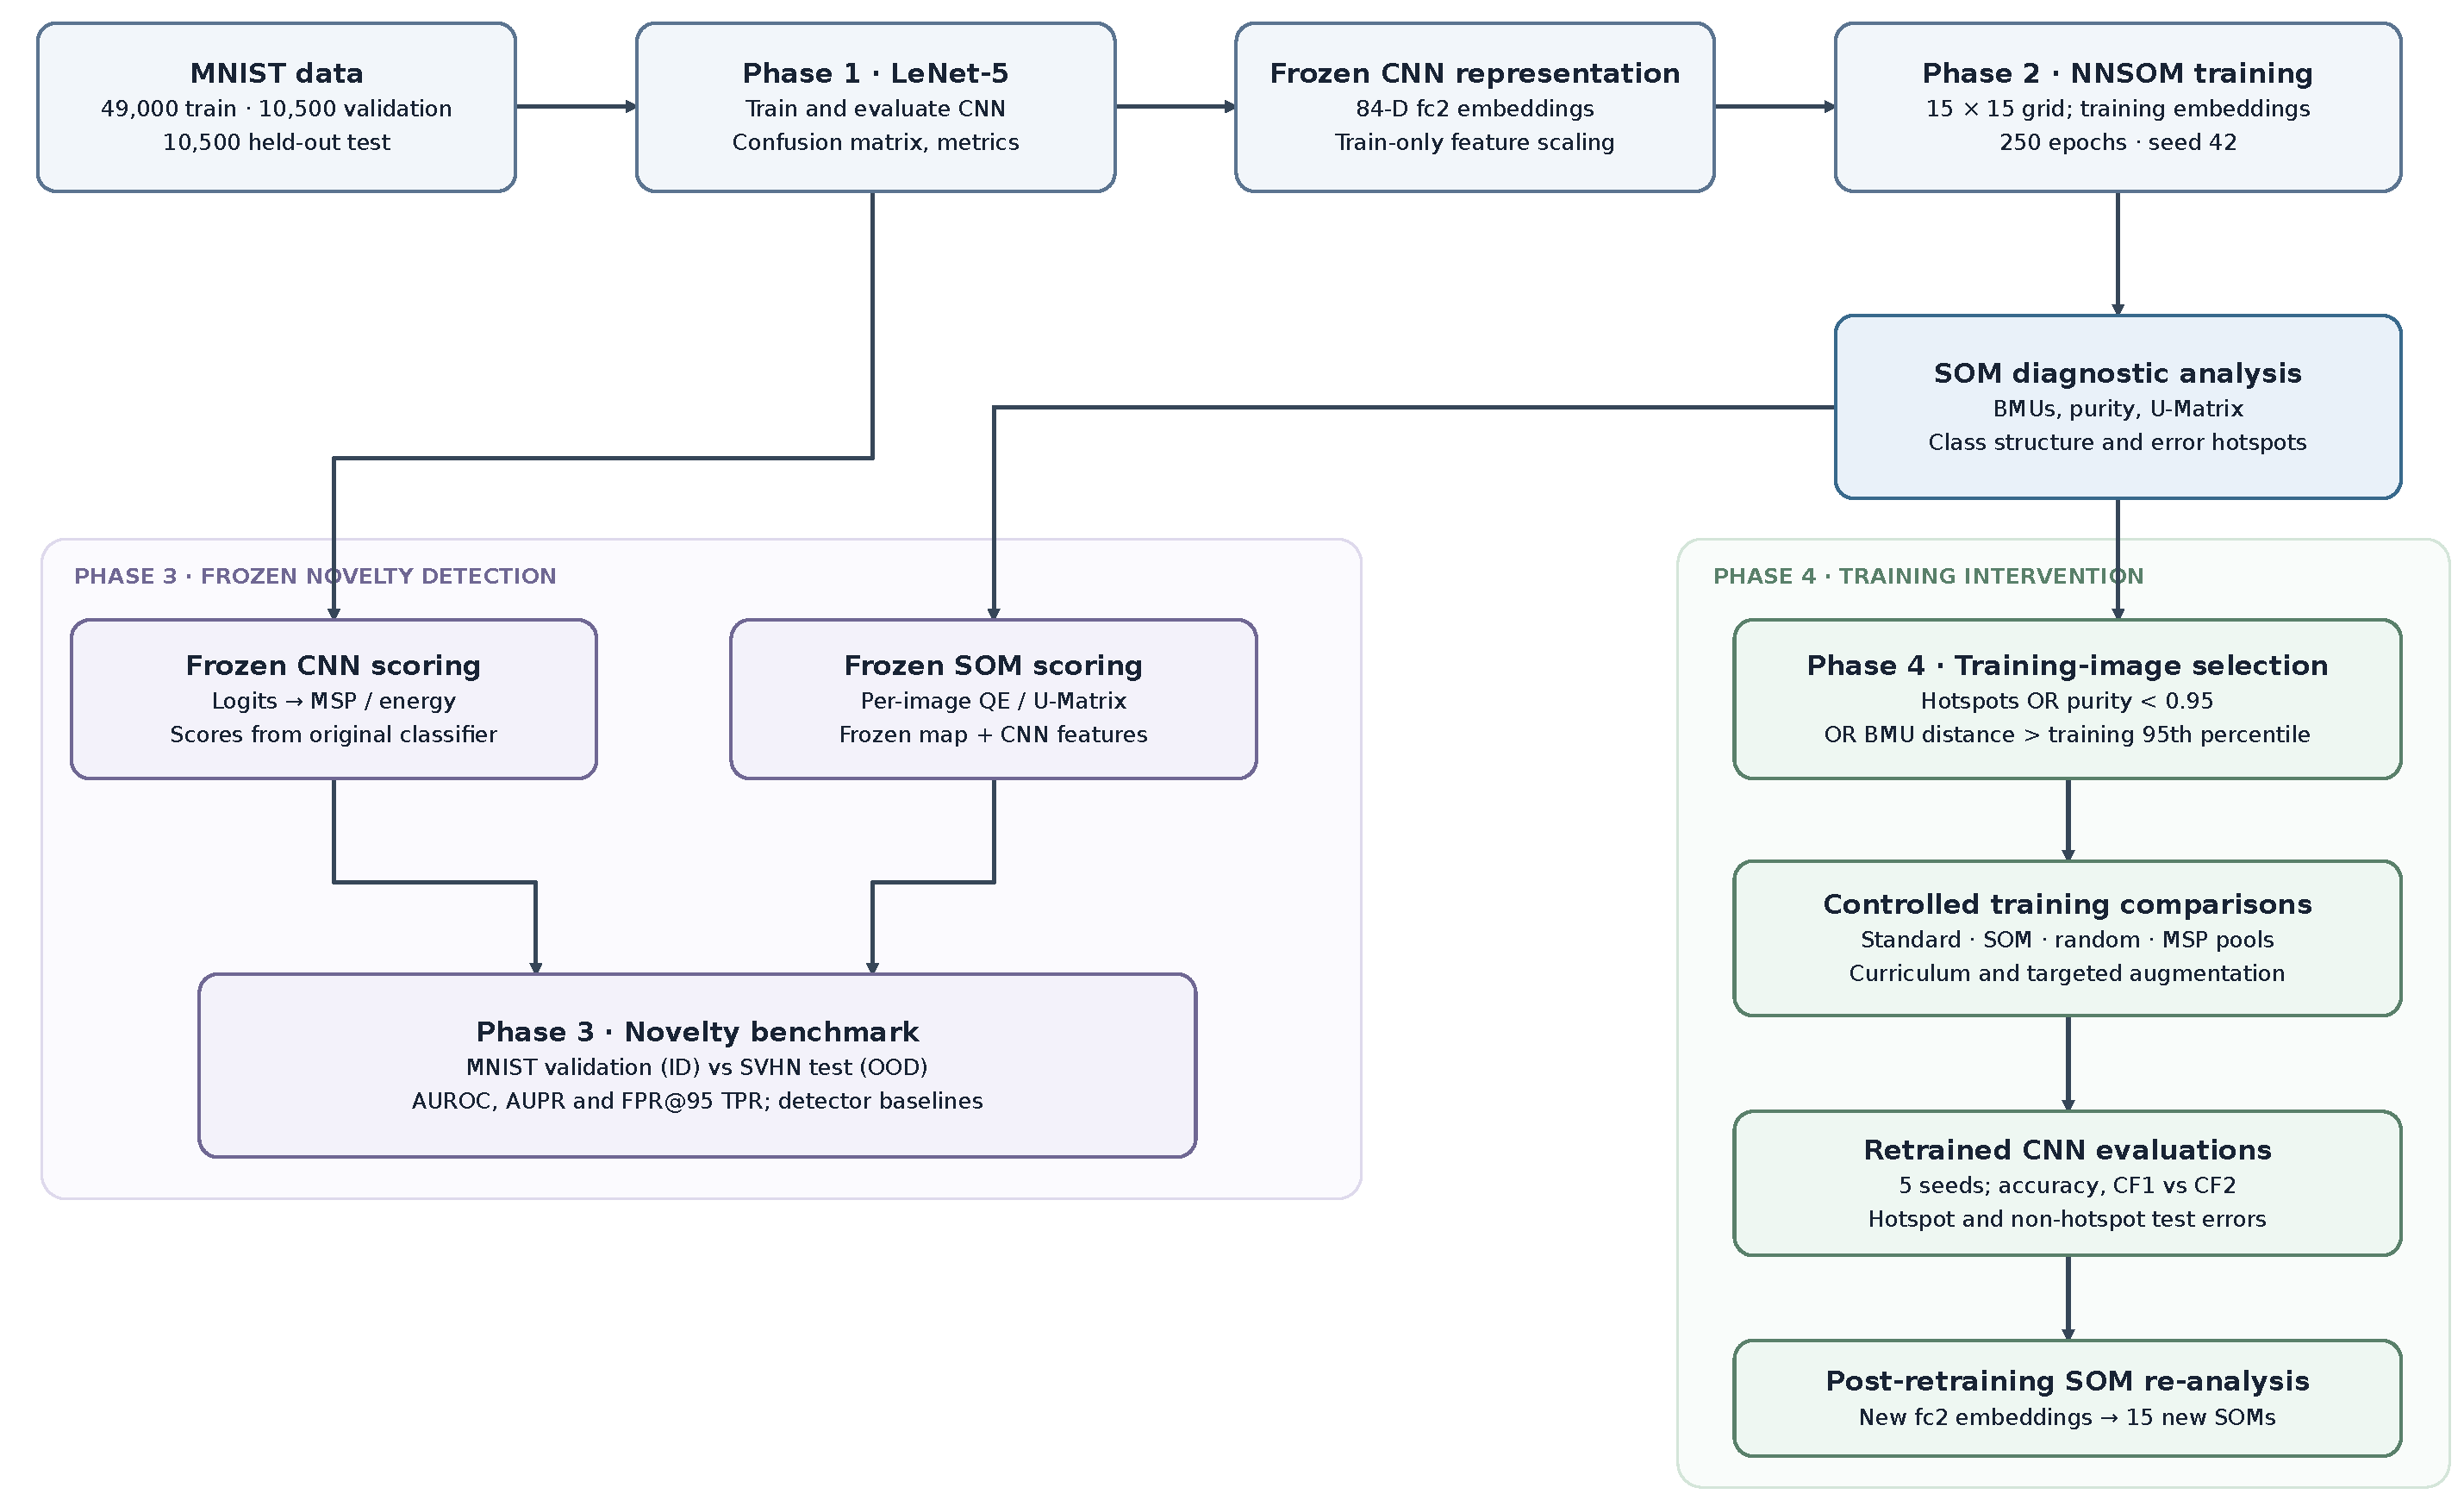
\includegraphics[width=\linewidth,keepaspectratio]{fig/pipeline/pipeline.pdf}
\caption{CNN--NNSOM post-training analysis workflow for MNIST. Frozen CNN representations support SOM diagnostics and separate novelty-scoring comparisons; SOM-derived training-example selection guides controlled CNN retraining and subsequent SOM re-analysis.}
\label{fig:workflow}
\end{figure}

\subsection{NNSOM training and the BMU}\label{sec:som}
A SOM comprises prototypes $w_j\in\mathbb{R}^{84}$ indexed by positions $r_j$ on a two-dimensional grid. Here the selected map has $15\times15=225$ units arranged on the recorded hexagonal topology. For a scaled embedding $z(x)$, the BMU is the closest prototype in Euclidean feature distance:
\begin{equation}\label{eq:bmu}
 b(x)=\underset{j\in\{1,\ldots,225\}}{\operatorname{arg\,min}}\,\lVert z(x)-w_j\rVert_2.
\end{equation}
\paragraph{Implementation-accurate batch training.}
The headline pipeline enables the recorded QE history and therefore uses the project's \texttt{train\_som\_with\_history} path, rather than directly calling NNSOM's native training loop. NNSOM supplies the SOM object, hexagonal neuron positions, initial prototypes (via \texttt{init\_w}) and plotting functions. An economy-SVD wrapper avoids constructing a full singular-vector basis during the package's initialization. The project code recomputes BMU assignments from the \emph{updated} prototypes at every epoch, a documented distinction from the tested native NNSOM 1.8.x behavior, which retained initial-weight winners after the first epoch. The custom path is a batch-prototype update, not the familiar online SOM learning-rate equation.

Let $z_i$ be scaled training embeddings, $b_t(i)$ their BMU under prototypes $w^{(t)}$, and $D_{jk}$ the NNSOM grid distance between neurons. With $t=0,\ldots,T-1$, $T=250$, the radius before each update is
\begin{equation}\label{eq:radius}
 \rho_t=1+(\rho_0-1)\left(1-\frac{t}{T}\right),\qquad \rho_0=11.
\end{equation}
A seeded Bernoulli mask $m_{it}\in\{0,1\}$ retains a winner with probability $0.90$. The implementation's neighborhood contribution to neuron $j$ is
\begin{equation}\label{eq:batchmembership}
 a_{jit}=m_{it}\left[\mathbf1\{D_{j,b_t(i)}\leq\rho_t\}+\mathbf1\{j=b_t(i)\}\right].
\end{equation}
The separate winner term reproduces the code's addition of the one-hot winner matrix to the neighborhood matrix; thus a retained winner contributes twice when it is also inside its own neighborhood. For $A_{jt}=\sum_i a_{jit}>0$ the prototype is assigned the neighborhood-weighted batch mean
\begin{equation}\label{eq:somupdate}
 w_j^{(t+1)}=\frac{\sum_i a_{jit}z_i}{A_{jt}},
 \qquad w_j^{(t+1)}=w_j^{(t)}\ \text{if }A_{jt}=0.
\end{equation}
Winners are recomputed after each epoch. The saved run uses training-only MinMax scaling to $[-1,1]$, a $15\times15$ grid, 250 epochs/steps and seed 42. Epoch-level NNSOM-style QE is recorded for convergence monitoring. These details follow the versioned training code; they should not be confused with an independently implemented stochastic gradient step. The pipeline records the input-embedding hashes, the training implementation, its model hash and its own run ID.

\paragraph{Grid choice and limitations.}
Three grid sizes (10$\times$10, 15$\times$15 and 20$\times$20) received comparable 250-epoch tuning budgets and within-grid neighborhood selection using validation features. Their held-out CNN-error-prediction comparison did not distinguish 20$\times$20 from 15$\times$15: difference $+0.001$ AUROC, interval $[-0.100,+0.089]$. The 15$\times$15 map, run \srcid{som_15x15_nb11_ep250_s42_v2}, is retained as the instructor-requested headline configuration, \emph{not} as a statistically established optimum. Grid-size robustness is reported separately rather than selected using test-set correctness.

\subsection{Map quality and visualization}
Quantization error requires distinguishing the \emph{per-image BMU distance} from the \emph{NNSOM map-level summary}. For each sample,
\begin{equation}\label{eq:qesample}
 s_{\mathrm{QE}}(x)=\lVert z(x)-w_{b(x)}\rVert_2.
\end{equation}
This individual distance is the novelty score, and its training 95th percentile defines the frozen OOD threshold. For a dataset $\mathcal D$, let $C_j=\{x\in\mathcal D:b(x)=j\}$ and let $K$ be the number of neurons. The NNSOM-style aggregate used for reported SOM quality and convergence is
\begin{equation}\label{eq:qe}
 \mathrm{QE}_{\mathrm{NNSOM}}(\mathcal D)=\frac{1}{K}\sum_{j=1}^K q_j,\quad
 q_j=\begin{cases}
 \displaystyle\frac{1}{|C_j|}\sum_{x\in C_j}s_{\mathrm{QE}}(x),&|C_j|>0,\\
 0,&|C_j|=0.
 \end{cases}
\end{equation}
Unlike the conventional sample-weighted mean, this summary first averages within each occupied neuron, assigns zero to empty neurons, and then averages across all $K$ neurons. The reported validation QE of 1.041 refers to this map-level definition; the OOD score distributions and cutoff refer to individual distances. Conflating these two statistics changes their interpretation.

First-order topographic error (TE1) is the percentage of images whose two closest prototypes have NNSOM topological distance greater than 1.1; first-plus-second-order TE uses a threshold of 2.1. Weighted neuron purity is the total occupancy-weighted fraction assigned to a neuron's modal true class, calculated only after unsupervised SOM fitting. Empty neurons are excluded from occupancy-weighted purity but contribute zero to the NNSOM aggregate QE.

The U-Matrix displays distances among neighboring prototypes. For grid neighborhood $\mathcal N(j)$, one local summary is
\begin{equation}\label{eq:umatrix}
 U_j=\frac{1}{|\mathcal N(j)|}\sum_{k\in\mathcal N(j)}\lVert w_j-w_k\rVert_2.
\end{equation}
Large neighboring-prototype distances suggest transitions between map regions; they do not prove that any particular sample is OOD. A hit histogram counts images assigned to each BMU. A class-dominance map indicates the modal class within each cell, while purity and entropy expose mixed regions. The validation error-geography map combines dominant true class, common incorrect prediction, and error concentration in one coordinate system. These visual encodings are useful for diagnosing regions, not for inferring causes of mistakes from topology alone.

\subsection{Error hotspots and comparator scores}
For each neuron the fraction of assigned images misclassified by the original CNN estimates its error rate. To reduce the influence of sparsely populated neurons, the recorded hotspot procedure ranks cells by the lower Wilson bound of their error rates \parencite{wilson1927probable}, with the number of selected cells defined as $\max(5,5\%\text{ of all neurons})$ (11 for the 15$\times$15 map). Hotspots are identified on one randomly selected half of the validation set and evaluated on the other, evaluated in both directions for 100 stratified half-split repetitions (200 held-out evaluations). The concentration ratio is
\begin{equation}\label{eq:ratio}
 R_{\mathrm{hot}}=\frac{\text{fraction of all CNN errors in hotspot cells}}{\text{fraction of all images in hotspot cells}}.
\end{equation}
An error concentration ratio of one corresponds to errors distributed proportionally to the number of samples; a ratio above one shows enrichment. Error-label shuffles form a null comparison. For error \emph{prediction}, we compare SOM neuron error rate with an occupancy-matched 225-cluster k-means scheme, impurity among nearby training embeddings and uncertainty from the CNN's maximum-softmax output. This classification-error task is distinct from the OOD task below; its AUROCs must not be mixed with OOD AUROCs.

\subsection{Novelty scoring and evaluation}\label{sec:oodmethod}
The MNIST-trained CNN and SOM are frozen during the main OOD comparison. MNIST validation images ($n=10{,}500$) are the in-distribution negative class; the official SVHN test images ($n=26{,}032$) are the external OOD positive class. SVHN is an OOD \emph{probe}, not a second trained classifier pipeline. The precommitted QE decision rule flags $s_{\rm QE}(x)>\tau$, where $\tau$ is the 95th percentile of MNIST training per-image BMU distances ($\tau\approx1.5690$). An example-level U-Matrix score summarizes neighboring-prototype separation around its BMU; it is not the same quantity as distance to the BMU.

We report AUROC, area under the precision--recall curve (AUPR, OOD positive), and false-positive rate at 95\% true-positive rate (FPR@95TPR). AUROC and FPR@95TPR describe rankings and operating points respectively; the training-quantile threshold's validation false-positive rate is a separate quantity. Comparisons include QE, U-Matrix, MSP, energy, $k$NN distance and Mahalanobis distance, plus documented historical Isolation Forest, One-Class SVM and autoencoder baselines. The newly fitted common-sample five-seed nine-method experiment is \emph{post-hoc exploratory}; its frozen-reference scores and freshly fitted baselines must not be interpreted as nine identically retrained models.

\subsection{Hard-example selection, retraining and new SOMs}\label{sec:retrainmethod}
The Phase 4 protocol uses SOM-based training-image selection: a training image is marked hard if its BMU is among the 11 hotspot units, its neuron purity is below 0.95, \emph{or} its BMU distance exceeds the training 95th percentile. This union yields 4,217 of 49,000 training images (8.6\%). The SOM-guided pool is compared with class-matched random selection and lowest-MSP selection. Targeted augmentation adds three transformed copies per selected image (reported ranges: rotations up to $10^{\circ}$, translation up to one pixel, zoom 0.9--1.1 and shear up to $8^{\circ}$). The curriculum experiments introduce hard examples progressively. The standard arm receives no added images, and five shared CNN seeds provide repeated paired comparisons. The Phase 4 test evaluation reports the original standard and retrained CNN predictions (CF1/CF2); no SOM/graph operator is inserted between a test image and its CNN prediction.

After selected retraining arms, the analysis extracts new 84-dimensional features and fits a new $15\times15$ SOM for each of three arms (standard, SOM augmentation and random augmentation) and five CNN seeds, yielding 15 new maps. These maps are evaluated on validation data for weighted purity, topology, error hotspots and other structure metrics. Their hotspot cells are selected again for each map, so the analysis describes \emph{different} BMU partitions and should not be misread as paired error rates on identical fixed map cells.

\section{Experimental Protocol and Leakage Control}\label{sec:protocol}
The initial CNN uses the recorded 49,000/10,500/10,500 train/validation/test split. Embedding scaling, the original SOM, and feature-space references are fitted on MNIST training representations. CNN checkpoint selection, grid comparison, map summaries and initial error-hypothesis development use validation data; they are not independent hold-out tests. The hotspot-concentration statistic uses split-half validation selection and evaluation, with shuffled-error nulls. The novelty study uses MNIST validation and SVHN as a \emph{development OOD evaluation}; it does not assert a new locked MNIST test assessment. The historical QE threshold comes from training QE, not SVHN performance. The Phase 4 comparison reports five seeds, standard, random and MSP controls, paired confidence intervals, prespecified criteria and a test evaluation; its map re-analysis is validation-only.

The initial 99.18\% CNN test accuracy is a \emph{single selected checkpoint}. Phase 4's 99.11\% ``standard'' mean is a \emph{different five-seed control}. Likewise, the Phase 2 split-half hotspot-concentration ratio of 11.1 is not the Phase 4 hotspot test error percentage. Comparisons retain their split, seed unit, definition and run identifier. The Phase 3 report documents unequal historical fitting budgets and the exploratory status of later common-sample experiments. Experiment provenance is carried by the frozen CNN checkpoint and feature hashes, the selected SOM run \srcid{som_15x15_nb11_ep250_s42_v2}, Phase 3 run-specific score files, and Phase 4 matched-seed arm summaries. The SOM training pipeline refuses mismatched frozen embeddings and rejects test-based selection; full runs use non-overwriting run-ID preflight and record model SHA-256. These code checks support auditability but are not equivalent to independently re-running every historical experiment. A changed augmentation transform was separately versioned after the original 2-pixel shift failed a validation check; the reported arms use the 1-pixel revision. No unmeasured post-retraining novelty AUROC is inferred.

\paragraph{Source and uncertainty register.} Table~\ref{tab:source_register} separates the experimental evidence by role and data split. These are references to existing recorded outputs, not claims that this manuscript recreated model training or independently recomputed all saved scores.
\begin{table}[htbp]\centering\footnotesize\setlength{\tabcolsep}{3pt}
\begin{tabular}{@{}p{0.24\linewidth}p{0.35\linewidth}p{0.32\linewidth}@{}}\toprule
Evidence & Primary recorded source & Evaluation / uncertainty\\\midrule
Initial CNN & Phase 1 CNN baseline, frozen \texttt{fc2} features & MNIST test; single checkpoint, Wilson interval\\
SOM topology and hotspots & \srcid{som_15x15_nb11_ep250_s42_v2}; Phase 2 grid/error reports & Validation; split-half repetition, error shuffle\\
OOD comparison & Phase 3 frozen QE/SVHN and separate baseline run records & MNIST val / SVHN; fixed-score bootstrap\\
Guided retraining & Phase 4 \texttt{arm\_results} and \texttt{criteria\_results} & MNIST test; five CNN seeds, paired image bootstrap\\
Re-trained SOMs & Phase 4 \texttt{reanalysis\_results} & MNIST validation; paired five-seed $t$ intervals\\\bottomrule
\end{tabular}
\caption{Provenance and statistical unit of the headline experiments. The Phase 3 exploratory nine-method fitting study is distinct from the frozen reference comparisons.}\label{tab:source_register}
\end{table}

\section{Results}\label{sec:results}
\subsection{Baseline CNN and SOM structure}
The original LeNet-5 correctly classifies 10,414 of 10,500 MNIST test images: 99.18\% accuracy (95\% Wilson interval 98.99--99.34\%), with macro-F1 0.9918. It makes 92 mistakes on validation images, compared with 86 on the test split. Figure~\ref{fig:baselinecf} shows the original test confusion matrix. Because MNIST error counts are small, even modest relative changes in error rate may represent few images.

\begin{figure}[htbp]\centering
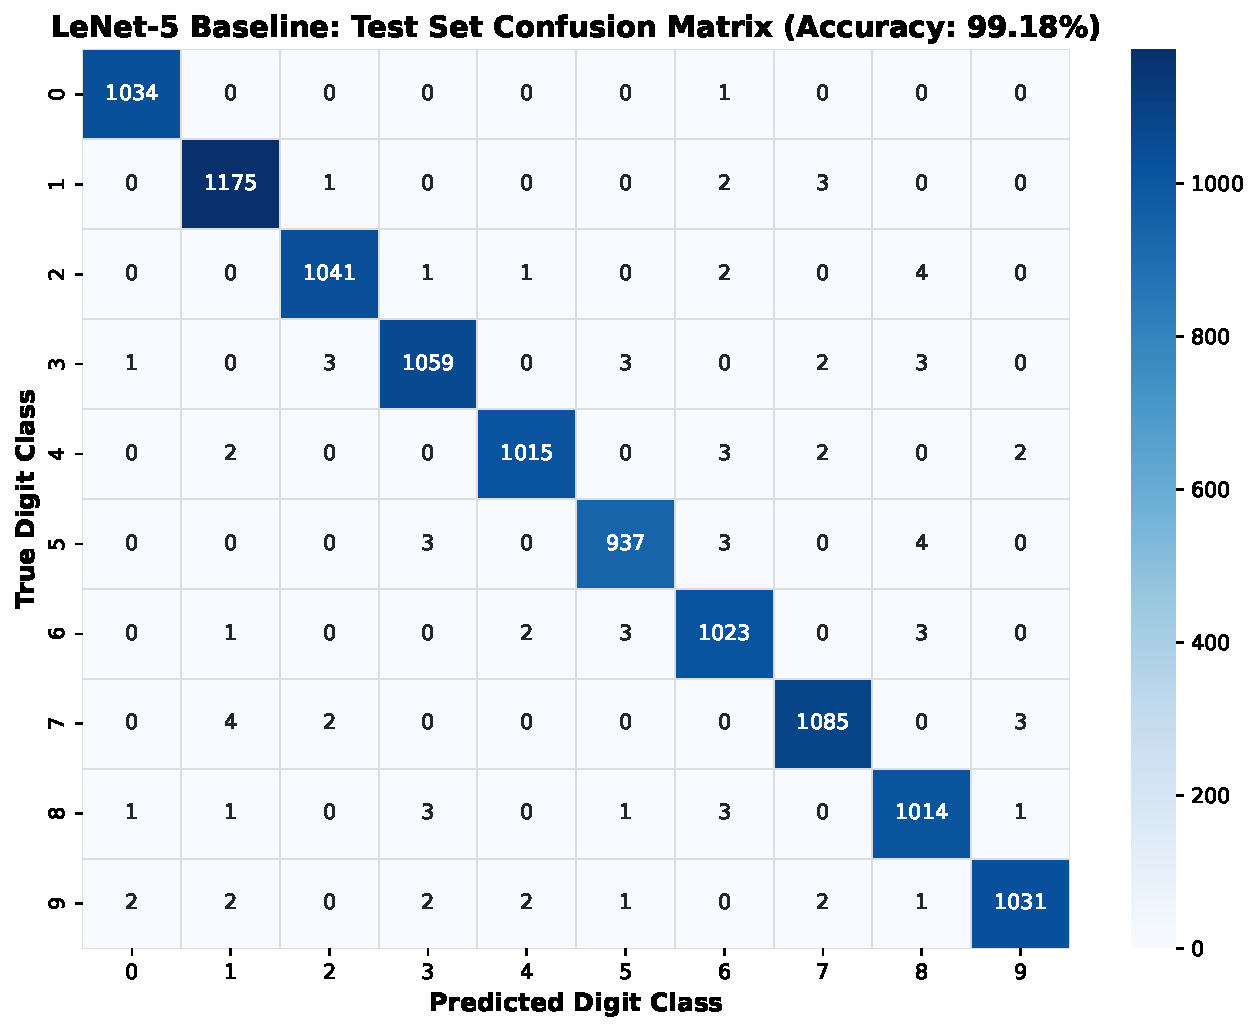
\includegraphics[width=0.78\linewidth,keepaspectratio]{p1_confusion_matrix.pdf}
\caption{Original LeNet-5 MNIST test confusion matrix ($n=10{,}500$, 99.18\% accuracy). This figure is from the original checkpoint, not the Phase 4 five-seed standard arm.}\label{fig:baselinecf}
\end{figure}

The headline 15$\times$15 SOM achieves validation QE 1.041, first-order topographic error 6.18\% and weighted class purity 98.19\%. Against shuffled labels, purity is approximately 17.4\% (95\% range 17.0--17.7\%, reported permutation $p=0.001$). The map therefore organizes the existing CNN representations by digit class, but class organization alone does not establish an improvement in error prediction. Figure~\ref{fig:geography} pairs the U-Matrix with validation error geography. On the left, local prototype separations reveal transitions in the learned topology: a larger distance indicates a more pronounced neighboring-weight change, not necessarily a classification mistake. On the right, the polygon face encodes the neuron\'s dominant true digit, the edge encodes the most common \emph{wrong} prediction among its errors, and edge width represents error concentration. Thus the right-hand image is not another U-Matrix: it overlays supervised validation diagnostics on an unsupervised map. The combined view supports spatial interrogation of errors, but apparent boundary proximity cannot by itself establish a causal explanation.

\begin{figure}[htbp]\centering
\begin{minipage}[c]{0.39\linewidth}\centering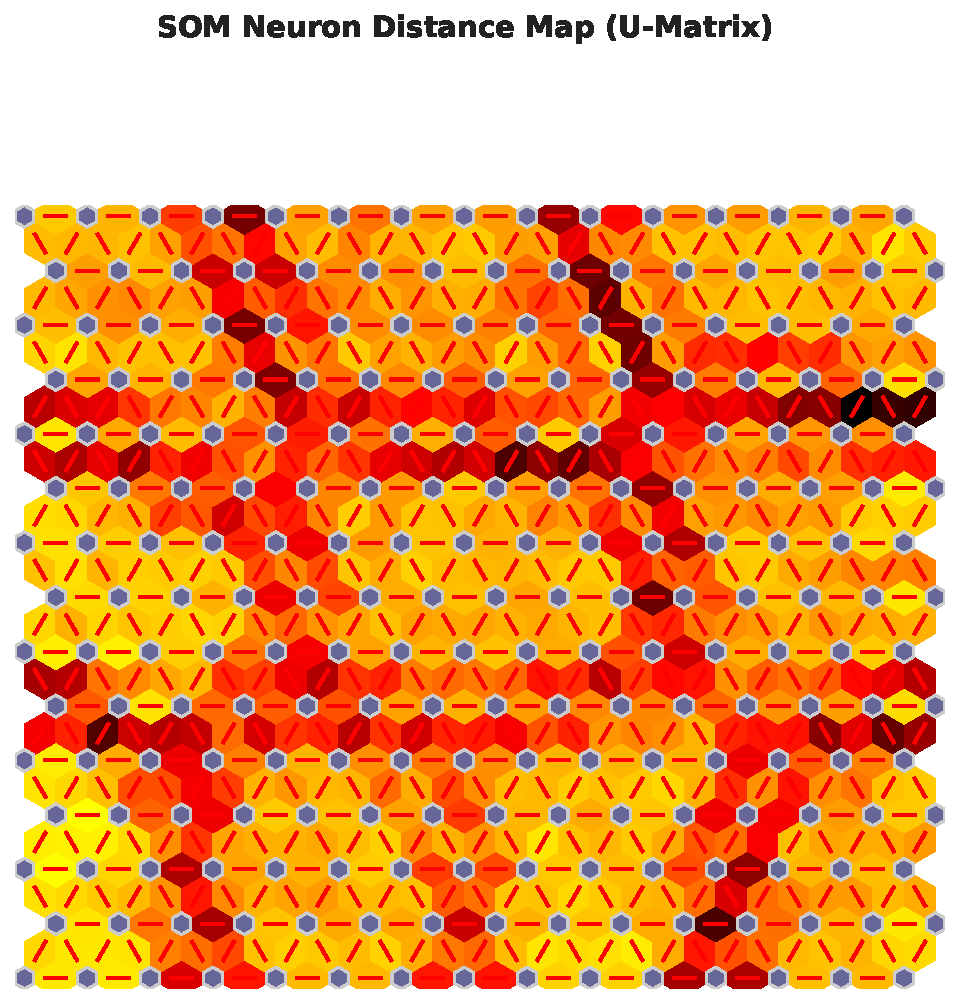
\includegraphics[width=\linewidth]{p2_u_matrix.pdf}\end{minipage}\hfill
\begin{minipage}[c]{0.59\linewidth}\centering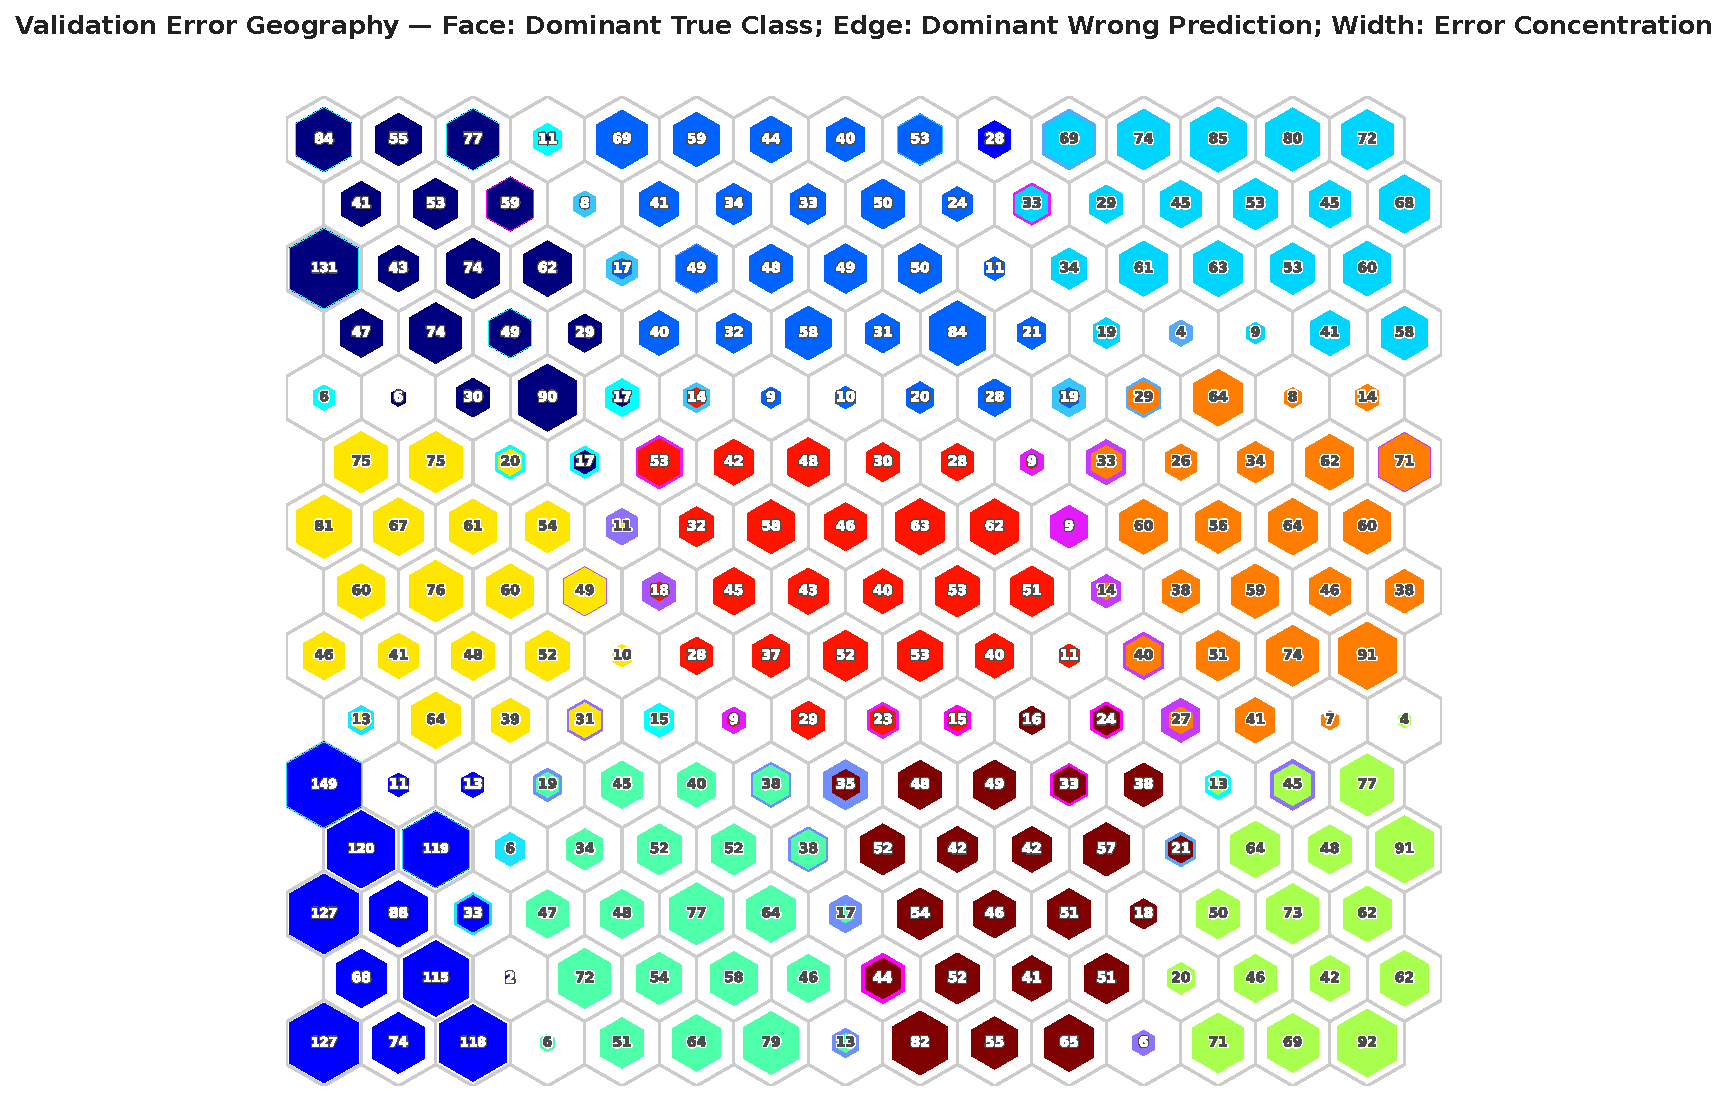
\includegraphics[width=\linewidth]{p2_validation_complex_error_map.pdf}\end{minipage}
\caption{SOM interpretation on MNIST. Left: U-Matrix of neighboring prototype distances. Right: validation error geography, encoding dominant true digit, typical wrong prediction and error concentration. The two views describe related but distinct map properties.}\label{fig:geography}
\end{figure}

\subsection{Error concentration and prediction baselines}
The 11 selected cells on the 15$\times$15 SOM contain errors at 11.1 times the concentration expected from their image share, according to the repeated split-half analysis (95\% range 6.1--17.6; shuffled-error $p=0.005$). Table~\ref{tab:phase2} preserves the existing three-grid comparison. The result is consistent with errors clustering near mixed class regions, but differences across grids are not decisive and the concentration ratios should not be interpreted as a ranking of grid quality.

\begin{table}[htbp]\centering\small\setlength{\tabcolsep}{4pt}\renewcommand{\arraystretch}{1.15}
\begin{tabular}{@{}lccc@{}}\toprule
Validation measure & 10$\times$10 & 15$\times$15 & 20$\times$20\\\midrule
Hotspot cells & 5 & 11 & 20\\
Concentration ratio (95\% range) & 10.5 (5.4--17.3) & 11.1 (6.1--17.6) & 13.4 (8.0--19.3)\\
Shuffle-null median & 0.98 & 0.94 & 0.93\\
Spearman: error vs. purity & $-0.755$ & $-0.810$ & $-0.766$\\
Spearman: error vs. entropy & $+0.778$ & $+0.816$ & $+0.768$\\\bottomrule
\end{tabular}
\caption{Original SOM grid comparison for 92 MNIST validation errors. All reported permutation $p=0.005$; concentration-ratio magnitudes should not be used to choose a grid.}\label{tab:phase2}
\end{table}

Table~\ref{tab:error-pattern-baselines} preserves the original comparison of \emph{classification-error prediction}, distinct from OOD detection. SOM cell error rate (AUROC 0.685) and the 225-cluster k-means score (0.693) are comparable; nearest-neighbor impurity (0.874) and CNN softmax uncertainty (0.981) perform better. The SOM's value is thus the reusable spatial account of where errors occur, not better numerical identification of individual errors.
{\setlength{\tabcolsep}{2.3pt}\begin{table}[H]
\centering
\renewcommand{\arraystretch}{1.15}
\small
\begin{tabular}{|p{0.20\textwidth}|p{0.17\textwidth}|p{0.095\textwidth}|p{0.13\textwidth}|p{0.09\textwidth}|p{0.09\textwidth}|}
\hline
\textbf{Score} & \textbf{AUROC (95\% range)} & \textbf{Avg. precision} & \textbf{Hotspot ratio} & \textbf{Images in hotspots} & \textbf{Errors in hotspots} \\ \hline
SOM 15$\times$15 cell error rate & 0.685 (0.624--0.738) & 0.053 & 11.1 (6.1--17.6) & 1.6\% & 18.1\% \\ \hline
k-means, 225 clusters, cell error rate & 0.693 (0.651--0.729) & 0.034 & 5.6 (4.6--6.1) & 3.8\% & 20.4\% \\ \hline
kNN impurity ($k=15$) & 0.874 (0.829--0.917) & 0.228 & -- & -- & -- \\ \hline
CNN max-softmax probability & 0.981 (0.974--0.987) & 0.336 & -- & -- & -- \\ \hline
\end{tabular}
\caption{How well each score finds the 92 validation images that the CNN gets wrong (10,500 images in total). AUROC ranges come from repeated half-splits for the cell scores, and from bootstrap resampling for kNN impurity and max-softmax. Hotspot ratio: share of mistakes divided by share of images in the 11 hotspot cells, chosen on one half and measured on the other. For k-means: median of 10 seeds, with the lowest and highest in brackets. Chance level is about 1 ($p=0.005$ for the SOM and for every k-means seed).}
\label{tab:error-pattern-baselines}
\end{table}
}

\subsection{Novelty detection: MNIST versus SVHN}\label{sec:oodresult}
The training-derived QE threshold is approximately 1.5690. At that threshold the historical evaluation flags 96.17\% of SVHN images while 5.13\% of MNIST validation images are flagged; these threshold-specific rates must not be confused with FPR@95TPR. Figure~\ref{fig:qedist} displays the distribution of \emph{individual} BMU distances for MNIST training and validation inputs, with a vertical threshold determined from the training set. The overlap illustrates that even familiar held-out images can exceed the cutoff; this panel contains no SVHN curve and cannot on its own demonstrate OOD discrimination. Figure~\ref{fig:svhnoverlay} then projects SVHN onto the frozen MNIST prototypes: occupancy identifies which neurons receive SVHN inputs, the middle panel gives the share missed under the fixed QE rule, and the final panel supplies the dominant MNIST class for interpretation. High occupancy is not the same as high detector confidence, and the three panels do not show that SOM outperforms scalar confidence methods.

\begin{figure}[htbp]\centering
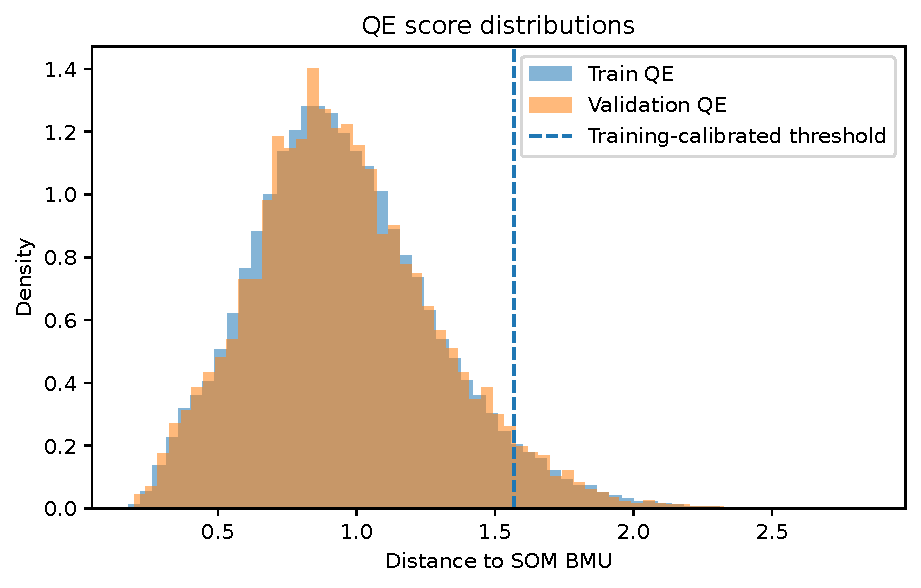
\includegraphics[width=0.73\linewidth]{p3_qe_score_distribution.pdf}
\caption{MNIST training and validation quantization-error distributions and the threshold fixed at the training 95th percentile. This is a calibration figure, \emph{not} a direct MNIST/SVHN ROC comparison.}\label{fig:qedist}
\end{figure}

\begin{table}[htbp]\centering\small
\begin{tabular}{@{}lccc@{}}\toprule
Scoring method & AUROC & AUPR & FPR@95TPR\\\midrule
Energy & \textbf{0.9998} & 0.9999 & \textbf{0.0004}\\
Maximum softmax (MSP) & 0.9985 & 0.9994 & 0.0078\\
SOM quantization error & 0.9811 & 0.9766 & 0.0453\\
$k$NN distance ($k=5$) & 0.9766 & 0.9739 & 0.0592\\
SOM U-Matrix & 0.9696 & 0.9865 & 0.0701\\
Mahalanobis distance & 0.7764 & 0.7859 & 0.3131\\\bottomrule
\end{tabular}
\caption{Recorded MNIST-validation ($n=10{,}500$) versus SVHN ($n=26{,}032$) OOD benchmarks. U-Matrix uses the historical five-method run (FPR@95TPR 0.0701); the additional CNN-score baselines are from the separate recorded frozen-CNN benchmark. These rows summarize fixed-model results and are not an equal-budget, jointly refitted six-method competition. Higher AUROC/AUPR and lower FPR@95TPR are better.}\label{tab:ood}
\end{table}

The paired fixed-score comparison finds $\mathrm{AUROC}_{\rm QE}-\mathrm{AUROC}_{\rm MSP}=-0.017388$ (95\% paired-bootstrap interval $[-0.019406,-0.015418]$, 2,000 resamples). Energy also outranks QE on the observed distributions. Original historical autoencoder and Isolation Forest rankings are below chance under their recorded score conventions; subsequent diagnostic fitting shows that standardizing embeddings materially changes autoencoder ranking. These historical and post-hoc experiments are not silently pooled into Table~\ref{tab:ood}. The Phase 3 diagnostic report records average embedding norms of approximately 40.3 for MNIST validation and 5.8 for SVHN, and a pooled Spearman association of approximately $-0.83$ between QE and norm. Restricting embeddings to the MNIST training-norm 5th--95th percentile range retained 9,447 MNIST validation examples but only \emph{eight} SVHN examples. The estimated QE AUROC on this tiny matched-range subset was 0.72 (reported interval [0.58, 0.84]), too uncertain for a general conclusion. This post-hoc diagnostic suggests substantial norm dependence without proving its causal origin or providing an independent new OOD benchmark.

\begin{figure}[htbp]\centering
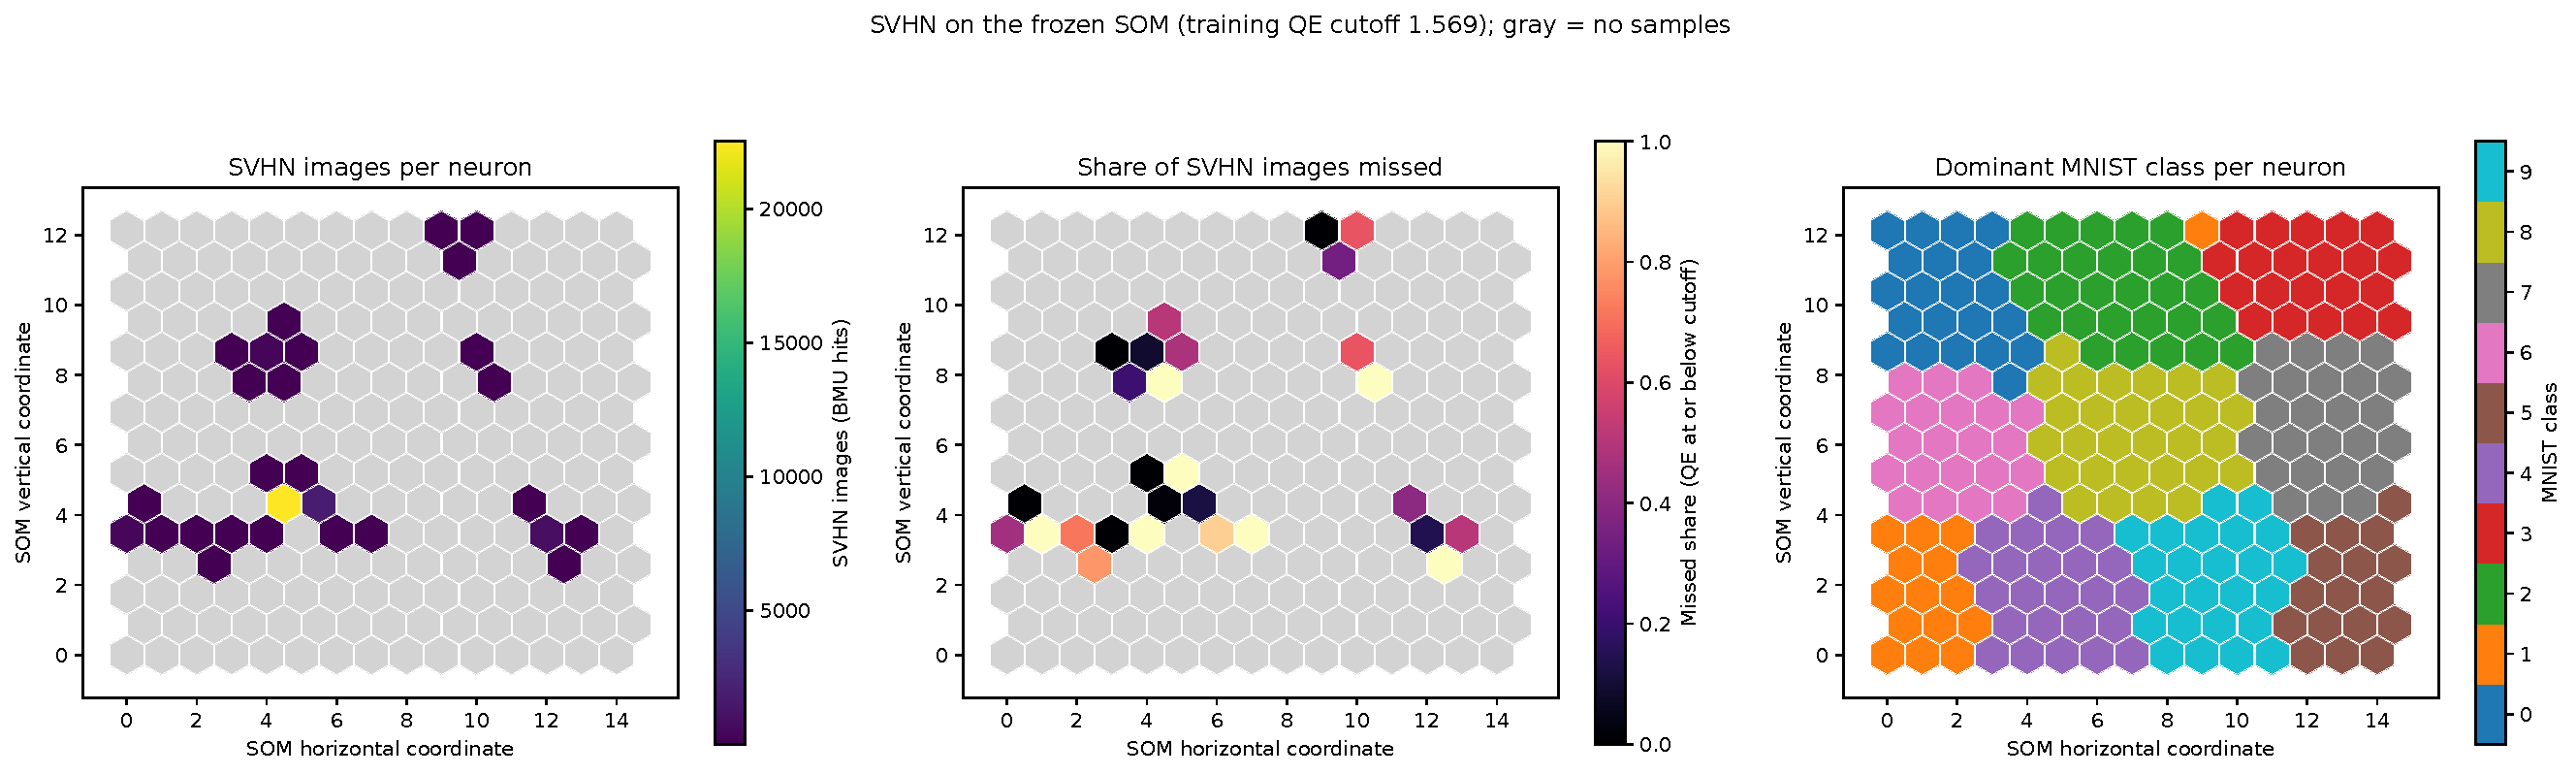
\includegraphics[width=0.96\linewidth]{p3_svhn_som_overlay.pdf}
\caption{SVHN locations on the frozen MNIST SOM: BMU occupancy (left), share of SVHN images missed at the frozen QE threshold (center), and modal MNIST class (right). The three aligned plots support error-geography interpretation but do not imply that map occupancy is a calibrated novelty probability.}\label{fig:svhnoverlay}
\end{figure}

\begin{figure}[htbp]\centering
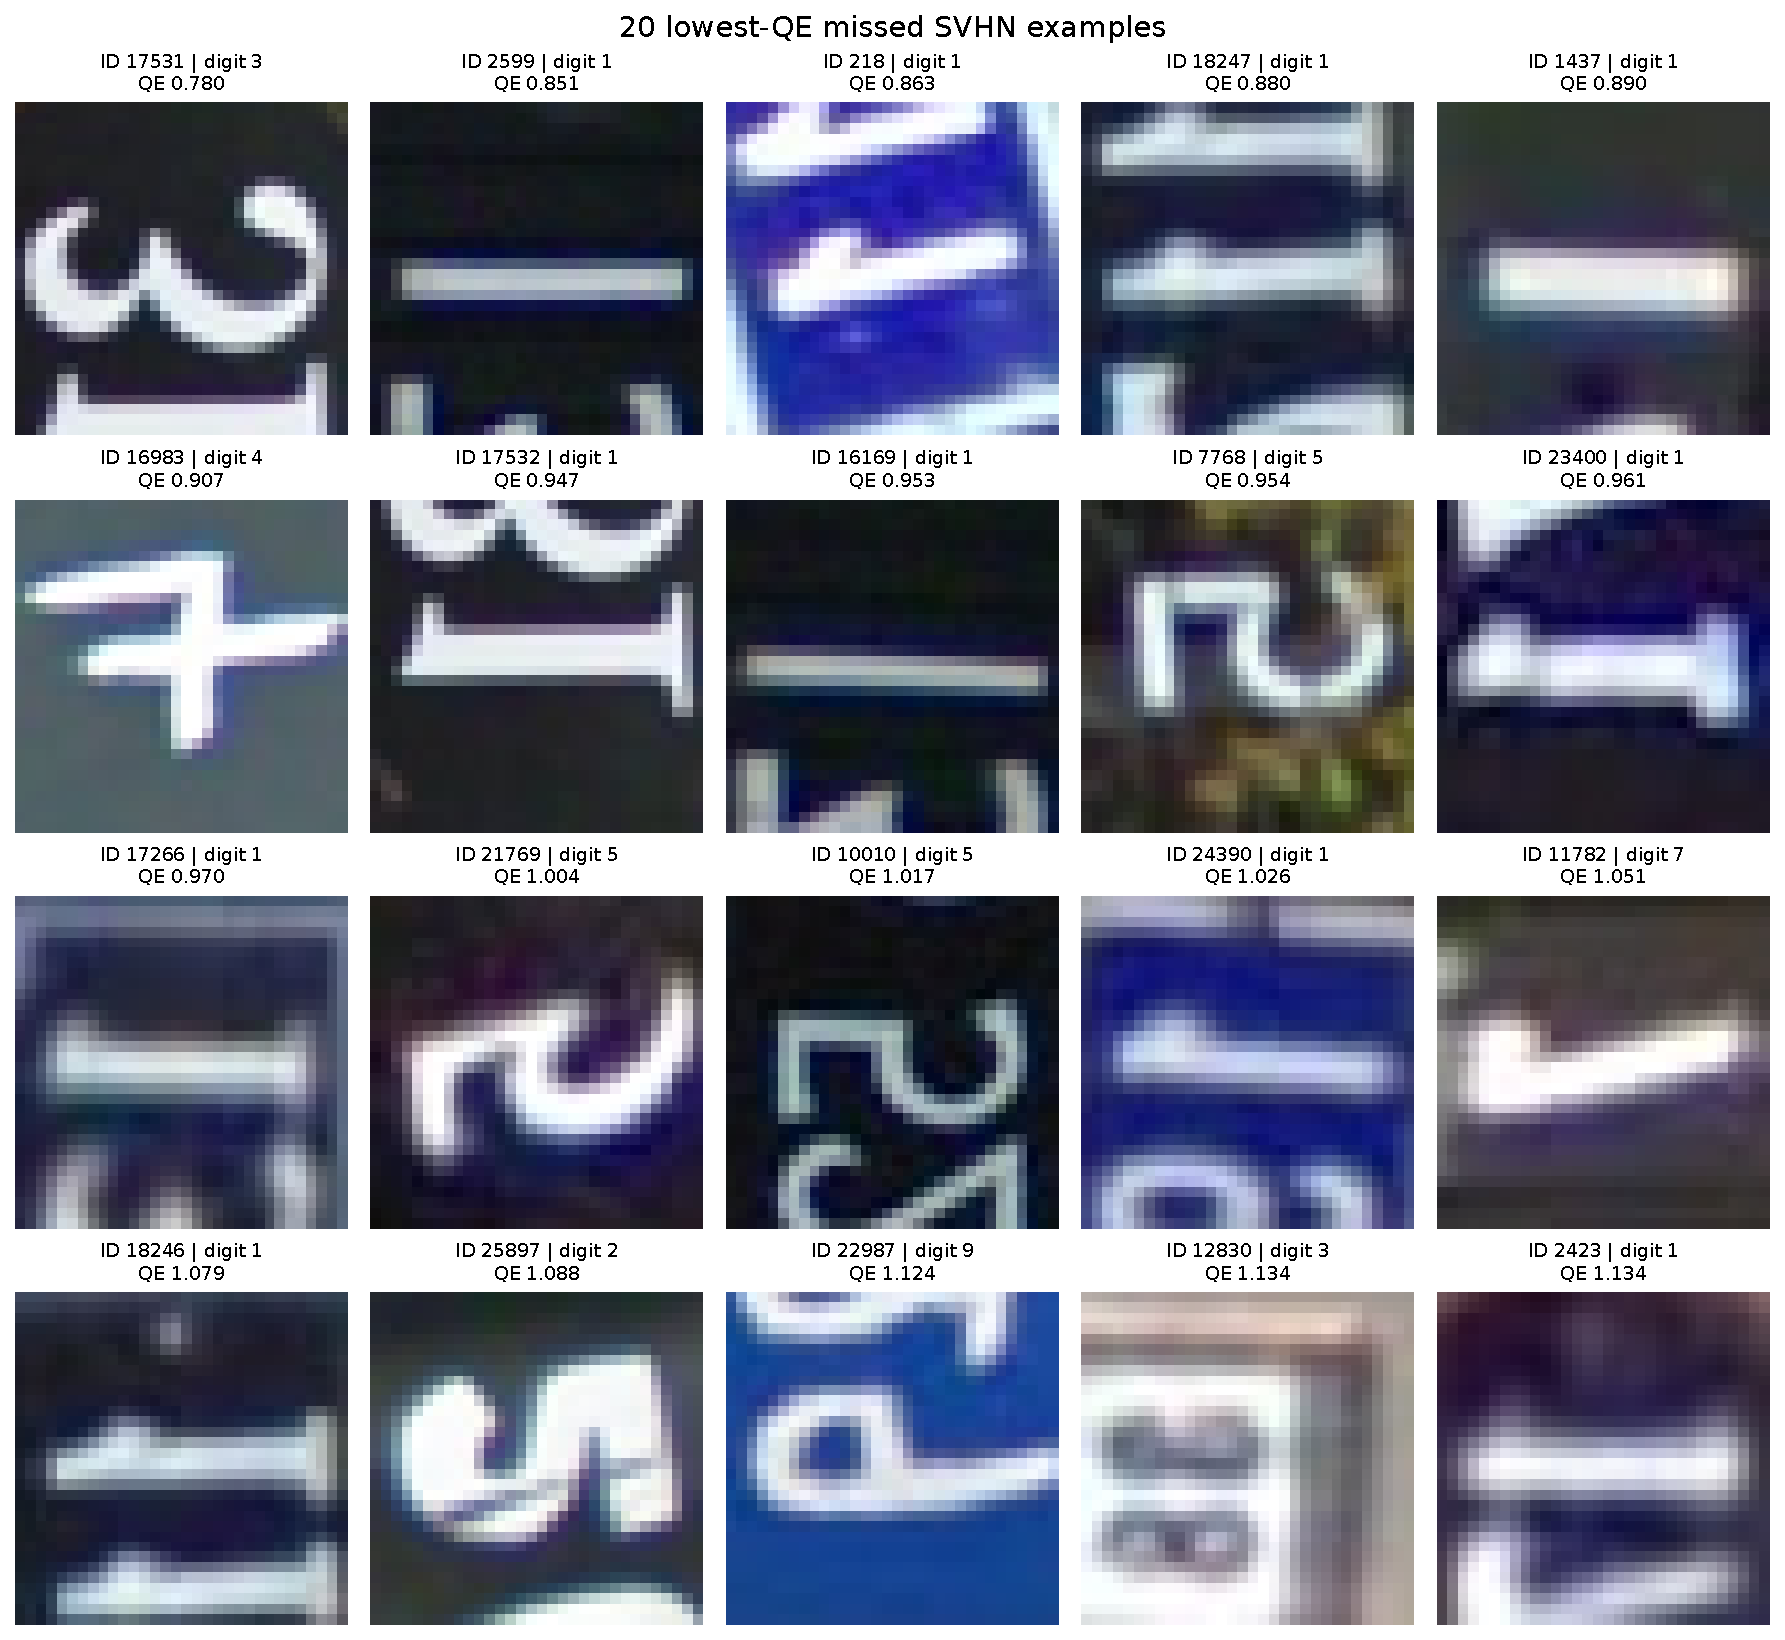
\includegraphics[width=0.75\linewidth]{p3_qe_missed_svhn_examples.pdf}
\caption{Twenty SVHN examples assigned low QE and missed at the fixed novelty threshold, demonstrating why a map-based detector should be evaluated against its misses as well as its overall AUROC.}\label{fig:oodmisses}
\end{figure}

\subsection{Guided retraining and classifier errors}\label{sec:retrainresult}
Table~\ref{tab:retrain} consolidates the completed five-seed test results. The original single-checkpoint accuracy of 99.18\% must not be substituted for the separate five-seed standard control of 99.11\%. Relative to this control, SOM-guided targeted augmentation improves mean overall test accuracy to 99.21\% and reduces the hotspot error rate from 11.4\% to 7.8\%. The MSP-guided arm has 99.25\% overall accuracy, while SOM-guided curriculum performs worse than standard training. These are means, not single-run maxima.

\begin{table}[htbp]\centering\small\setlength{\tabcolsep}{6pt}
\begin{tabular}{@{}lccc@{}}\toprule
Training arm & Accuracy (\%) & Hotspot error (\%) & Outside hotspots (\%)\\\midrule
Standard (CF1) & 99.11 (0.12) & 11.4 (2.6) & 0.74 (0.10)\\
SOM augmentation (CF2) & 99.21 (0.07) & \textbf{7.8 (2.6)} & 0.69 (0.05)\\
Random augmentation & 99.18 (0.05) & 10.3 (2.4) & 0.68 (0.05)\\
MSP augmentation & \textbf{99.25 (0.06)} & 8.5 (1.2) & 0.64 (0.06)\\
SOM curriculum & 98.66 (0.04) & 21.4 (2.9) & 1.05 (0.06)\\\bottomrule
\end{tabular}
\caption{Test results: mean (standard deviation) across five CNN seeds. The 146 hotspot test images and 10,354 non-hotspot images use the recorded Phase 4 hotspot definition. Other arms are documented in the source Phase 4 report.}\label{tab:retrain}
\end{table}

Figure~\ref{fig:cfphase4} shows standard-training and SOM-augmentation mean confusion matrices across the five shared CNN seeds, together with their signed difference. Fractional entries in the difference matrix are averages over independent runs rather than literal fractions of an image. Figure~\ref{fig:augment} illustrates the label-preserving transformations used to construct three additional training copies per selected example; it does not by itself establish that a transformation improves accuracy.\par
The prespecified Phase 4 comparisons find a hotspot error difference of $-3.56$ percentage points for SOM augmentation versus standard training (95\% CI $[-5.75,-1.37]$), and $-2.47$ points versus random augmentation (CI $[-4.52,-0.68]$). Against MSP augmentation the estimated difference is $-0.68$ points (CI $[-2.88,+1.23]$), insufficient to distinguish the two methods. Outside-hotspot error does not increase beyond the protocol's stated tolerance. These confidence intervals are based on the report's paired bootstrap and are different uncertainty objects from the sample SDs shown in Table~\ref{tab:retrain}.

\begin{figure}[htbp]\centering
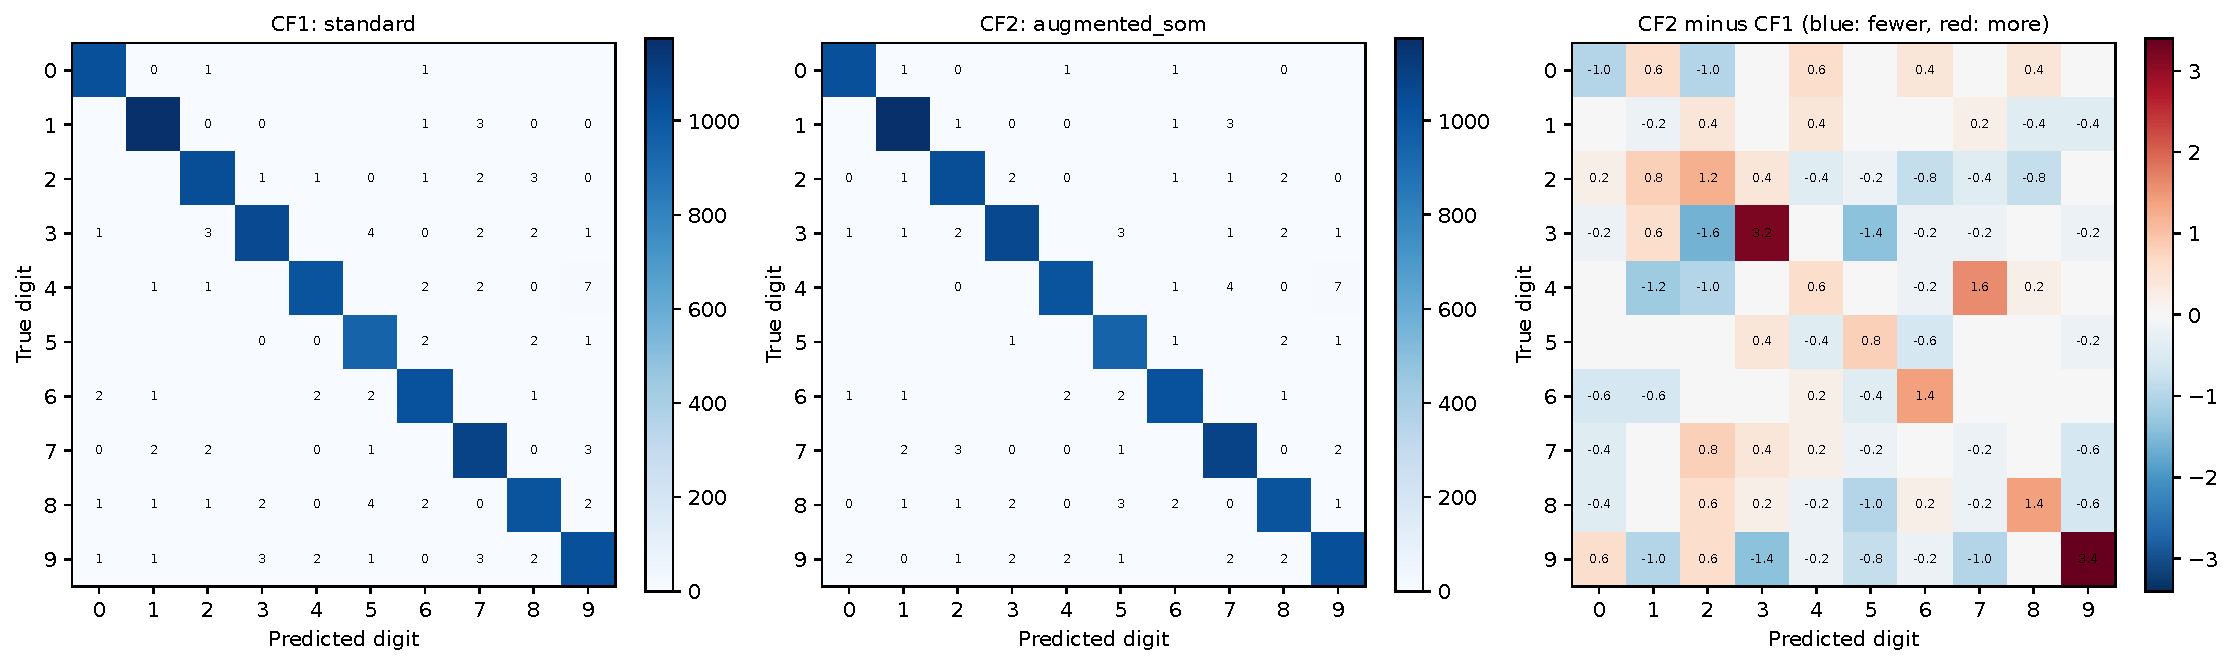
\includegraphics[width=\linewidth]{p4_confusion_standard_vs_augmented_som.pdf}
\caption{Phase 4 CF1 (five-seed standard training), CF2 (five-seed SOM augmentation) and their mean confusion-matrix difference on MNIST test images. The SOM determines the augmented training pool; it is not a test-time classifier stage.}\label{fig:cfphase4}
\end{figure}

\begin{figure}[htbp]\centering
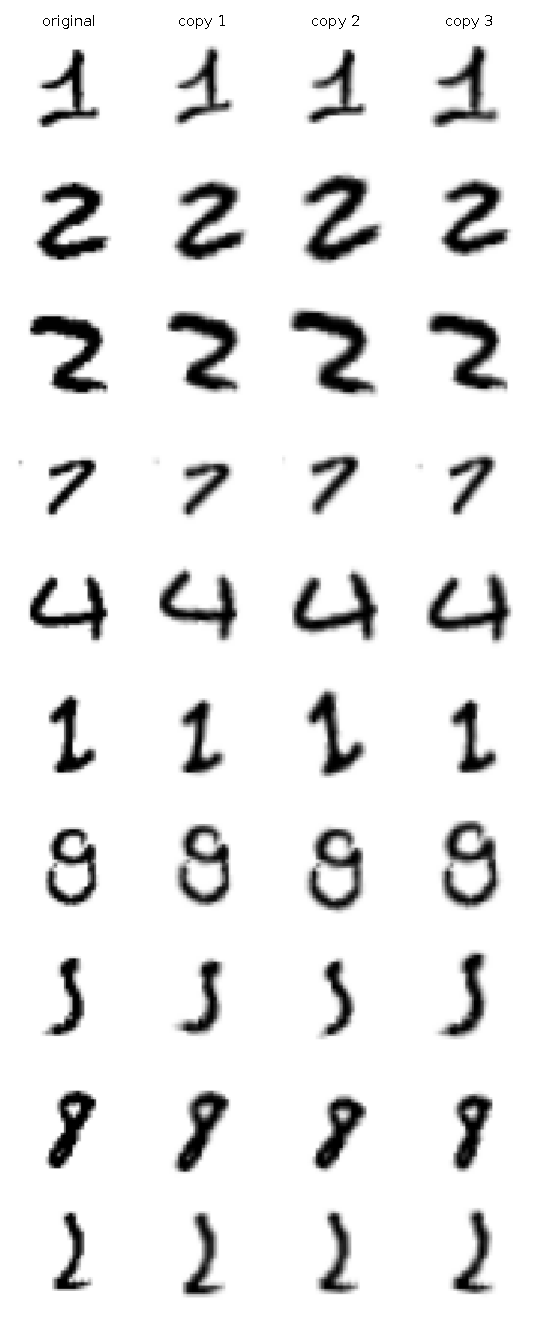
\includegraphics[width=0.52\linewidth]{p4_augmentation_contact_sheet.pdf}
\caption{Examples of training images selected for augmentation and three altered copies of each, illustrating the intervention applied to hard-example pools. The panel is illustrative, not an accuracy comparison.}\label{fig:augment}
\end{figure}

\subsection{Re-analysis after retraining}\label{sec:reanalysis}
The new SOM comparison evaluates map structure on validation data for five CNN seeds and three retraining arms. Each re-trained CNN generates fresh 84-dimensional embeddings, to which a new 15$\times$15 SOM is fitted using the original SOM recipe; the original Phase 2 map is only a reference. This produces 15 new SOMs, with a fixed SOM seed but five distinct CNN seeds. Table~\ref{tab:reanalysis} is a compact extraction of the supplied Phase 4 re-analysis results. SOM-guided augmentation reduces the new map's mean hotspot error relative to standard retraining; a comparison to random augmentation is less conclusive. Weighted neuron purity does not show a clear increase, so narrower failure regions should not be described as globally cleaner class separation. In Figure~\ref{fig:purity}, color represents each independently fitted map\'s validation class purity and red outlines mark its own selected hotspots. A particular location in the original map is not guaranteed to represent the same prototype or the same subset of images in the post-retraining maps. The figure supports qualitative within-map inspection; quantitative arm differences come from Table~\ref{tab:reanalysis}, not visual cell-by-cell subtraction.

\begin{table}[htbp]\centering\small\setlength{\tabcolsep}{4pt}
\begin{tabular}{@{}lccc@{}}\toprule
Validation metric & Standard & SOM aug. & Random aug.\\\midrule
Weighted neuron purity & 0.9824 & 0.9824 & 0.9813\\
Topographic error (\%) & 7.04 & 6.76 & 6.66\\
Hotspot error rate & 0.2292 & 0.1746 & 0.2061\\
Overall error rate & 0.0092 & 0.0075 & 0.0086\\\bottomrule
\end{tabular}
\caption{Summary of the post-retraining SOM validation study (means over five CNN seeds). SOM-minus-standard hotspot error is $-0.0545$ (95\% paired $t$-interval $[-0.1008,-0.0082]$); SOM-minus-random is $-0.0315$ ($[-0.0705,+0.0075]$). Hotspots are reselected separately for each fitted SOM.}\label{tab:reanalysis}
\end{table}

\begin{figure}[htbp]\centering
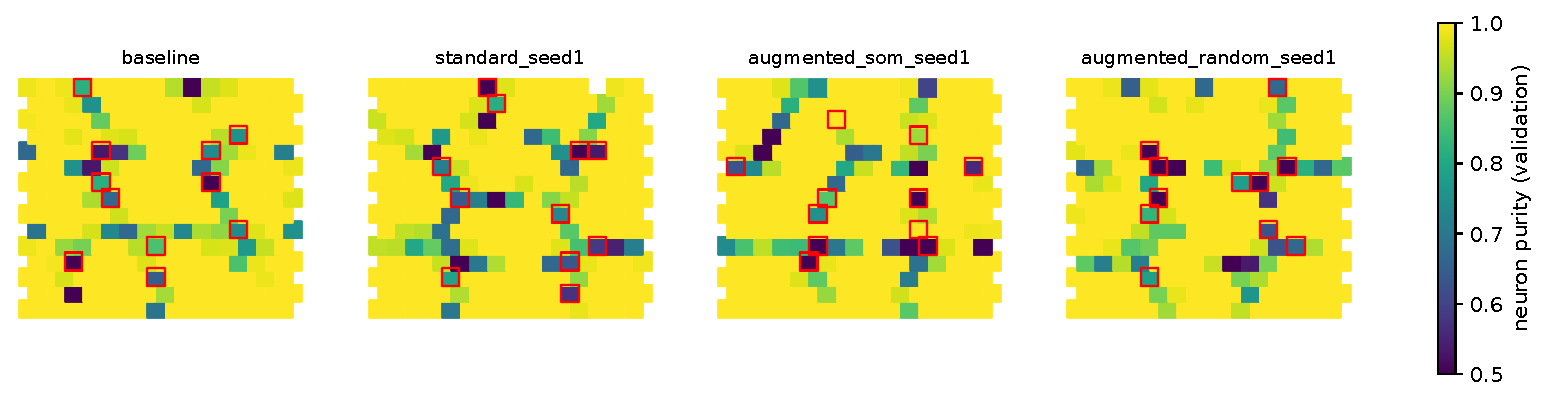
\includegraphics[width=0.95\linewidth]{p4_purity_maps.pdf}
\caption{Validation neuron purity for the original SOM and representative standard, SOM-augmented and random-augmented models (seed 1). Red outlines mark the hotspot neurons of each map, which are not necessarily the same image subsets.}\label{fig:purity}
\end{figure}

\section{Discussion and Limitations}\label{sec:discussion}
\textbf{What the SOM makes visible.} The MNIST embeddings form class-consistent regions of a fixed two-dimensional map; ambiguity and errors concentrate in a relatively small subset of units. This representation allows an analyst to display class dominance, prototype distance, wrong-prediction structure and novel-input arrivals in a common coordinate system. The analysis thus provides a navigable view of \emph{where} failures occur, while it does not establish a causal account of \emph{why} any particular image is misclassified.

\textbf{Predictive comparisons constrain the claim.} For error prediction, k-means produces a similar AUROC, while simple CNN softmax uncertainty is substantially stronger. For OOD ranking on MNIST validation versus SVHN, energy and MSP exceed SOM QE. The QE--MSP paired interval is below zero. Our results therefore support SOM as an explanatory and diagnostic complement, not as a leading detector. The OOD analysis also reveals sensitivity to cross-dataset embedding-norm differences; the exploratory norm-restriction test contains only eight external OOD examples in the retained range. Strong discrimination on SVHN therefore cannot be generalized to unknown inputs with comparable embedding magnitudes. The frozen QE cutoff and the ROC-derived FPR@95TPR describe different operating points, and the additional historical baselines did not share identical training budgets.

\textbf{Intervention has mixed evidence.} SOM-guided augmentation reduces hotspot test errors relative to standard and matched random training under the Phase 4 protocol. Yet MSP-guided augmentation remains statistically competitive, and the curriculum schedule underperforms. The new SOMs exhibit lower hotspot error after SOM augmentation than after standard retraining, without clear global purity improvement. New hotspots are reselected for each map, precluding a literal same-cell before/after interpretation.

\textbf{Internal validity and generalization.} The project uses a high-accuracy MNIST classifier with few remaining errors; hotspot comparisons use only 146 test examples in the recorded Phase 4 definition. The original checkpoint and retraining controls are different experiments. The Phase 3 SVHN benchmark is a development comparison, later common-sample fits are post-hoc exploratory, and some historical baselines used different training budgets. The original map uses a single SOM seed, while five-seed Phase 4 intervals describe CNN seed variability rather than a full distribution of independently retrained SOM initializations. Phase 4 hotspots are defined from SOM partitions, so hotspot-focused evaluation can favor SOM-guided selection; moreover, the re-analysis reselects hotspots separately within each map. The prespecified augmentation criteria and paired controls strengthen the within-experiment inference but cannot remove these scope limitations. Checkpoint selection also depends on validation data. These limitations restrict claims about other models, datasets, run-to-run SOM stability and general deployment conditions.

\paragraph{Interpretation boundary.} The spatial map shows \emph{where} a CNN\'s existing representation places hard examples; a topological boundary is neither an explanation of a particular pixel-level confusion nor evidence that an input is unsafe or alien. Because original MNIST accuracy is already above 99\%, few residual errors remain, and several confidence-based alternatives offer stronger numerical detection. The defensible contribution is a common geometry for diagnosis, novelty inspection, and intervention assessment, accompanied by explicit negative and inconclusive comparisons.

\section{Conclusion}\label{sec:conclusion}
We integrated frozen-CNN feature analysis, SOM topology, error-hotspot evaluation, OOD detection, guided augmentation and SOM re-analysis into a single MNIST study. The 15$\times$15 NNSOM map organizes the network's embeddings into interpretable class regions and identifies non-random concentrations of errors. QE is informative for distinguishing the examined MNIST validation and SVHN sets but does not outperform the classifier's MSP or energy scores. SOM-guided augmentation improves the studied hotspot error rates over standard and random controls, while MSP-guided selection remains competitive and curriculum learning does not help. The supported contribution is a transparent, spatial framework for analyzing failure regions and evaluating targeted responses, rather than a claim of superior classification or OOD detection accuracy.

\paragraph{Scope of evidence.} Novelty AUROC following guided retraining was not measured in the reviewed experiments and is not inferred. The findings are restricted to the recorded MNIST-trained classifier, its frozen NNSOM representation, the SVHN external OOD probe and the documented five-seed retraining comparisons. Broader claims require independent data and implementation-level replication.

\clearpage
\printbibliography[title={References}]
\end{document}
